% Generated by plsimcount.pfgrouping -- do not edit; regenerate instead.
% Suzuki S2, total, unmerged, cz, seed 1, t = n, measured r
% git_commit=8c69e76829985cb586945dc9e8ed58101f318fe1 git_dirty=False
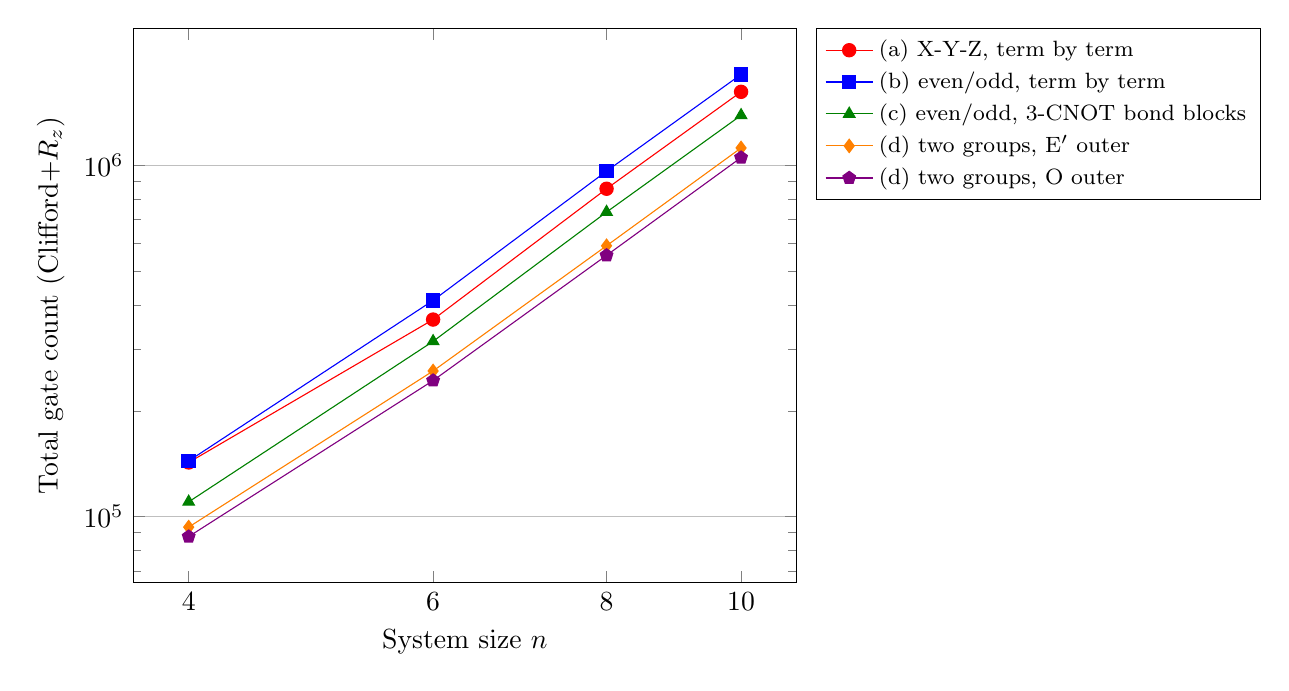
\begin{tikzpicture}
  \begin{loglogaxis}[
    width=10cm,
    xlabel={System size $n$},
    ylabel={Total gate count (Clifford+$R_z$)},
    xtick={4,6,8,10},
    xticklabels={4,6,8,10},
    ymajorgrids=true,
    legend pos=outer north east,
    legend cell align=left,
    legend style={font=\footnotesize},
  ]
    \addplot[red, mark=*, mark size=2.4pt, mark options={solid, fill=red}] coordinates {
      (4,142596)
      (6,363834)
      (8,857616)
      (10,1618740)
    };
    \addlegendentry{(a) X-Y-Z, term by term}
    \addplot[blue, mark=square*, mark size=2.4pt, mark options={solid, fill=blue}] coordinates {
      (4,144024)
      (6,412488)
      (8,962472)
      (10,1814580)
    };
    \addlegendentry{(b) even/odd, term by term}
    \addplot[green!50!black, mark=triangle*, mark size=2.4pt, mark options={solid, fill=green!50!black}] coordinates {
      (4,110136)
      (6,315432)
      (8,736008)
      (10,1387620)
    };
    \addlegendentry{(c) even/odd, 3-CNOT bond blocks}
    \addplot[orange, mark=diamond*, mark size=2.4pt, mark options={solid, fill=orange}] coordinates {
      (4,93340)
      (6,259740)
      (8,590200)
      (10,1120600)
    };
    \addlegendentry{(d) two groups, E$'$ outer}
    \addplot[violet, mark=pentagon*, mark size=2.4pt, mark options={solid, fill=violet}] coordinates {
      (4,87718)
      (6,243939)
      (8,554124)
      (10,1051945)
    };
    \addlegendentry{(d) two groups, O outer}
  \end{loglogaxis}
\end{tikzpicture}
